%---Document Class---%
\documentclass[12pt,final]{report}

%---Packages---%
\usepackage[a4paper, margin=1.2in]{geometry} %Document settings
\usepackage{authblk} %Title
\usepackage{graphicx} %Figures

\usepackage[hidelinks]{hyperref} %Emails in Title
\usepackage{sectsty} %Change fonts
\usepackage{tocbibind}
\usepackage[usenames,dvipsnames]{xcolor} %Colors
\usepackage{listings} %Code
\usepackage{amsmath} %Equations
\usepackage{mathtools} %More equations
\usepackage{caption}
\usepackage{subcaption}
\usepackage{ifdraft}
\usepackage{tikz}
\usepackage{gnuplot-lua-tikz}

% Externalize tikz pictures to speed up compilation if not in "final" mode.
% Requires pdflatex to be called with -shell-escape.
\ifoptionfinal{}{%
	\usetikzlibrary{external}\tikzexternalize
}

\renewcommand*\rmdefault{lmss} %font
\chapterfont{\color{NavyBlue}}   % sets colour of chapters
 % sets colour of chapters
\sectionfont{\color{Black}}  % sets colour of sections
\subsectionfont{\color{Gray}}  % sets colour of sections



%---Begin Document---%
\begin{document}

	%!TEX root = ../report.tex

% Title Page
\title{Path planning for paths that keep object in sight}
\date{May 30, 2015}
\author{Jorge Rodriguez\thanks{\href{mailto:jorod14@student.sdu.dk}{jorod14@student.sdu.dk}}}
\author{Ignacio Torroba\thanks{\href{mailto:igtor14@student.sdu.dk}{igtor14@student.sdu.dk}}}
\author{Kim Schwaner\thanks{\href{mailto:kschw10@student.sdu.dk}{kschw10@student.sdu.dk}}}
\author{Carlos Moro\thanks{\href{mailto:camor14@student.sdu.dk}{camor14@student.sdu.dk}}}
\affil{University of Southern Denmark\\Faculty of Engineering}

	\maketitle
	\begin{abstract}
A workcell consisting of a PA10 robot with a tool mounted stereo rig and surrounded by walls has been programmed to perform three-dimensional path generation for keeping a target inside the field of view of the cameras. 
The resulting algorithm, created and implemented in ROS, is composed of a structure of nodes whose inputs are the pairs of images acquired by the cameras and that outputs the robot joint configurations required to safely follow the target.
In the vision side, the target detection in both rectified images is carried out, leading to a triangulation process in which the 3D position of the target is accurately extracted with respect to the stereo rig.
The extracted coordinates are after used to compute the future position of the target based on its physical model by means of a Kalman filter. 
Once obtained, both positions are utilized in the robotics side of the project to carry out the path planning.
The desired, collision-free position of the camera rig is computed from the target position, and the necessary displacement calculated in the joint configuration space applying inverse kinematics. 
Before executing the displacement, a collision detector and a path optimizer algorithms are employed. 
However, if the straight line trajectory contains obstacles, an RRT-planner finds a safe different path between configurations.\\
The system has been successfully tested in both simulation and the workcell, and subjected to experiments to measure the magnitude of the errors in the performance. 
It has proved robustness and reliability, although certain limits imposed by the robot conditions have constrained the goodness of the final results.






\end{abstract}
	\tableofcontents

	%!TEX root = ../report.tex

\chapter{Introduction}
\label{chap:introduction}

\section{Overall description}
The present report contains the description of the  project "Path planning for paths that keep
object in sight" developed as a part of the course RoVi2: Robotics and Computer Vision 2. 
The aim of the developed system is to enable the existing setup consisting of a PA10 with a tool mounted stereovision system to safely plan the required three-dimensional trajectories for keeping a specific user-controlled target within the field of view of its cameras at any moment. 

\section{Report structure}
The project has been divided into two well differentiated parts. On one side the computer vision part, under which the recognition of the target, its tracking and location and the modeling of its physical behavior are treated. On the other side the robotics part, which gathers all the processes in charge of the trajectory planing and collision detection for the robot.

The described structure if applied to the report as well ***.
	%!TEX root = ../report.tex
\chapter{ROS Nodes Structure} % (fold)
\label{chap:ros_nodes_structure}

% chapter ros_nodes_structure (end)
	%!TEX root = ../report.tex
Section\section{Feature extraction} % (fold)
\label{sec:feature_extraction}
The goal of this chapter is to explain how the target object is detected in both images. With these positions the stereopsis can be computed as explained in \ref{sec:stereopsis} and hence the 3D position of the target in the world can be obtained.
The tracking of the object is a function implemented inside the node "balltracker" explained in section \ref{sec:structure}.

\subsection{Methods}
The underlying problem of the feature extraction is providing a feature strong enough that avoids correspondence problems such as occluding edges, homogeneous areas and repetitive structures.
In the case of occluding edges, the main problem is that a feature in the border of the object for one camera usually matches another one from the other camera (specially for round or cylindrical objects) although they are not the same point.
On the other hand, the problem with homogeneous areas is that all the patches of a smooth surface with a constant illumination look exactly the same and can be mismatched.
Finally, the problem of repetitive surfaces affects mainly when it comes to matching images containing structures like fences or buildings which are usually very repetitive and can lead to mismatch features because they look too similar.
To avoid these problems, it was decided to use a ball as the target object.
The reason for this is that the whole area of the surface of the ball can be seen by each camera and, hence, its centroid detected, completely avoiding the occluding edges and the homogeneous surfaces. What is more, the ball itself is not a repetitive structure, so that doesn't produce a problem either.

To achieve a reliable detection of the target in both images it was decided to use the contour finder provided by OpenCV.
For doing so a binary image is need as an input for the contour finder as this function uses the algorithm in \cite{suzuki}. 
The binary image is obtained by first converting the input image from RGB to HSV colorspace.
The reason for this is that the last one provides an easier way of tracking colours more complex than the pure red, green or blue.
Then, the proper values for the hue, saturation and value are obtained by trial and error and then the 3 channels are thresholded, producing binary image that can be seen in figure \ref{fig:binary_image}.
However, this process yields some artefacts in the image that need to be removed for the contour finder not to detect too many unnecessary contours.
 
\begin{figure}[h]
    \centering
    %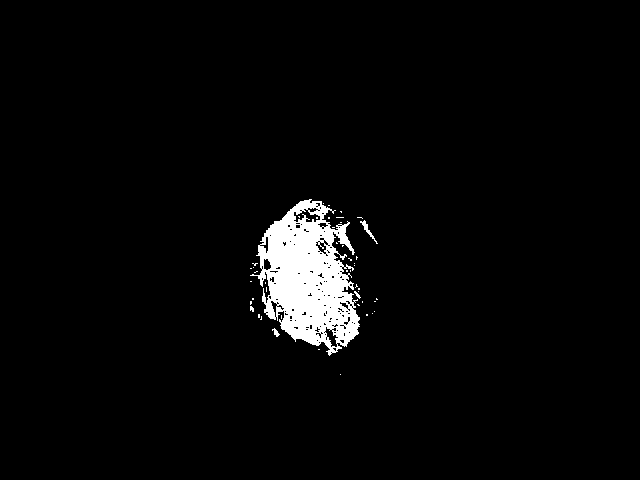
\includegraphics[width=0.8\textwidth]{images/binary.png}
    \caption{Binary image obtained after applying color threshold}
    \label{fig:binary_image}
\end{figure}

For removing those artefacts two morphological operators are applied. First of all an opening operation with a square kernel of 9x9 pixels that removes the small artefacts spread across the image and keeps the target intact. After this, a closing operation is perform with the same kernel. In this case, the aim of this is reducing the size of the gaps that appear inside the target after the thresholding in order to get a solid object. The result of this process can be seen in figure \ref{fig:filtered_image}.

\begin{figure}[h]
    \centering
    %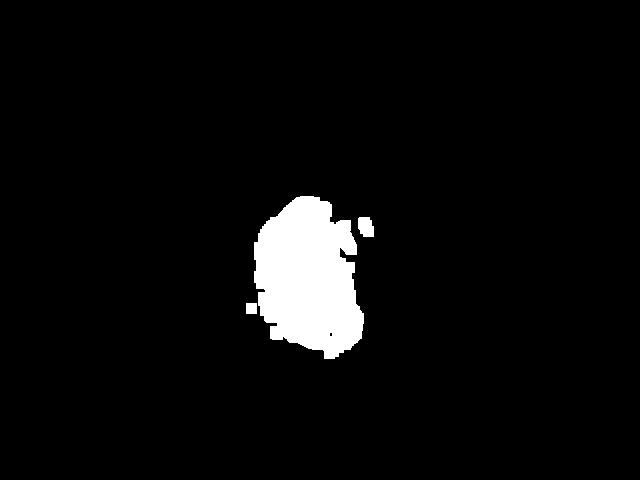
\includegraphics[width=0.8\textwidth]{images/filtered.png}
    \caption{Binary image obtained after applying the morphological operations}
    \label{fig:filtered_image}
\end{figure}

After removing the smallest objects from the binary image and closed the gaps in the remaining ones the finding contours function is applied, which provides an array with the detected contours. Following, the area and the outer perimeter of all the contours are computed. With these values, a radius threshold is applied so that only the contours with enough radius are accepted. For doing so, the equations for the perimeter and the area of a circumference are applied as it can be seen in equations \ref{eq:circ_perimeter} and \ref{eq:circ_area}.

\begin{equation}
perimeter_{contour}>2*\pi*radius_{threshold}
\label{eq:circ_perimeter}
\end{equation}

\begin{equation}
area_{contour}>2*\pi*radius_{threshold}^{2}
\label{eq:circ_area}
\end{equation}

Following, the circularity of the contours that have a radius bigger than the specified threshold is computed following equation \ref{eq:circularity}, which gives a value between 1 and 0 (being 1 a perfect circle, and 0 a straight line). Having this value computed, a threshold for the circularity is set so that only the target passes it. Finally, the moments of the remaining contour (the target) are calculated so that the centroids can be computed according to equation \ref{eq:centroids}. Then, this values are returned so that the stereopsis function can compute the 3D points for the target.

\begin{equation}
circularity=\frac{4*\pi*area_{contour}}{perimeter_{contour}^{2}}
\label{eq:circularity}
\end{equation}

\begin{equation}
centroid_{X}=\frac{m_{10}}{m_{00}} \qquad centroid_{Y}=\frac{m_{01}}{m_{00}}
\label{eq:centroids}
\end{equation}

\subsection{Results}
Several variations of the algorithm stated above were tested before ending up with that one. However, the original ball given as a marker to be tracked was completely white. Therefore, as the laboratory where the workcells are situated has high ceilings and the only windows are close to them, the sun was hitting with a high angle. This illumination configuration produced very bright spots on the top of the ball (easily seen by the cameras) while the rest of the ball stayed with less brightness. In addition, the walls surrounding the workcell are mainly white and, at certain moments of the day very bright. Consequently, tracking the white ball was a very difficult task. To fix this issue, the ball was covered with a piece of green paper that made the colour detection easier. Nevertheless, the high inclination of the sun still produced a spot of higher brightness in the top of the ball that wasn't detected by the algorithm. For fixing this, the closing morphology operation was performed as explained in the section above, which provided a much circular shape to the ball in the image than the one obtained by simply thresholding.
All in all, the final detection of the ball was stable enough to provide consistent data for the stereopsis and the trajectory prediction.

% section feature_extraction (end)~\ref{sec:}
	%!TEX root = ../report.tex

\chapter{Stereovision} % (fold)
\label{chap:stereopsis}

\section{Introduction}
In this section, the solution adopted for the location of the target in the 3D space through the vision system, the reasons that led to this approach, the assumptions made and the obtained results are presented. 
A more detailed explanation of the 2D image processing performed for the target tracking can be found in \ref{chap:feature_extraction}.

\section{Stereopsis}
Due to the fact that two vision systems were available on the setup, the first step was to decide which one to employ and the method to compute disparity. 
After a slight evaluation of resources the chosen one was the stereo rig, utilized to carry out sparse stereo with a single well-defined point. 
Thus, the next points contain the steps to compute the position of a point in 3-space given its image in two views and the camera matrices. 

Through the acquired pairs of images, the pixel coordinates of the center of gravity of the target are extracted by the algorithm presented in \ref{chap:feature_extraction}. 
They are used to calculate its 3D coordinates referred to the camera reference frame by means of linear triangulation methods.

\section{Camera model}
As a consequence of the need of a defined relation between the image and the object space, the cameras must be used as a mapping. 
The mathematical model assumed for the camera is the basic pinhole structure, described in \cite{Hartley}. 
This model defines a linear projection from the 3D world to the image plane, and contains the intrinsic parameters that relates the camera and the image reference frames as showed in equation \ref{eq:pinhole_model}. Where X represent the homogeneous coordinates of a 3D point and x its projection in the image plane in pixel coordinates.
 
\begin{equation}
x = P·X
\label{eq:pinhole_model}
\end{equation}  

Since the linearity assumed by this model does not hold due to imperfections in the lens, a distortion model needs to be added to the calculations in order to correct the deviations on the real cameras. 
The Plumb Bob distortion model, introduced in \cite{Brown} is applied here since it is the one used by ROS.

\subsection{Camera calibration}
\label{sec:cam_calib}
In order to obtain the intrinsic parameters for the camera model, a stereo calibration process based on a 2D pattern has been carried out for both Bumblebee2 1394a cameras by means of a ROS node. The procedure and some basics of it are to be found in \ref{sec:camera_calibration}.

\section{3D Reconstruction}
In order to compute the depth for a pair of correspondent image points, a suitable triangulation method light but robust enough to be executed on line with sufficient accuracy must be found. 
The task, trivial in theory, entails certain complexity due to the acquisition errors in the measured image coordinates. 
An immediate, simple approach could consists in back-projecting the correspondent image points, by means of the projection matrices, and finding the 3D point in the space in which they intersect. 
However, this procedure is very unlikely to succeed in most of the cases since the image points do not satisfy the epipolar constraint due the errors.

\begin{figure}[h]
    \centering
   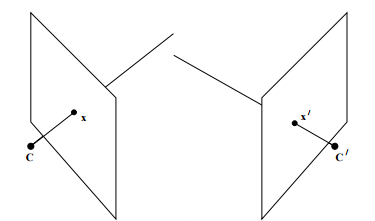
\includegraphics[width=0.8\textwidth]{figures/back_projection}
    \caption{Back-Projection rays error}
    \label{fig:Back-Projection}
\end{figure}

This is because in most of the cases the rays will not intersect in the 3D point, since there is not a point X that satisfies the equations \ref{eq:projection}. 

\begin{equation}
	\centering
	x  = P·X  $$\\
	x' = P'X $$
	\label{eq:projection}
\end{equation} 

\subsection{Triangulation}
The applied method to estimate depth and compute the estimations of 3D positions is the defined for the OpenCV functions utilized in the developed algorithm. 
This method is based on the direct linear transformation procedure to compute the estimation of the 3D point.

\subsubsection{Direct Linear Transformation}
The equations \ref{eq:projection} are combined into a set of linear equations in X of the form \ref{eq:DLT} by eliminating the scale factor, where the matrix A is \ref{eq:DLT2}

\begin{equation}
	\centering
	AX = 0 
	\label{eq:DLT}
\end{equation}

\begin{equation}
A =
 \begin{pmatrix}
  xP^{3T} - P^{1T} \\
  yP^{3T} - P^{2T} \\
  x'P^{'3T} - P^{'1T} \\
  yP^{'3T} - P^{'2T}
 \end{pmatrix}
 \label{eq:DLT2}
\end{equation}

The way the DTL algorithm solves this set of redundant equations in the unknowns of X is by means of a Least-squares minimization problem in the absence of an exact solution. 
The presence of noise reduces the problem to the minimization of \ref{eq:LSM} where e stands for the projection errors.
The LS solution solution is given in equation \ref{eq:LSM_solution}.

\begin{equation}
	\centering
	\lVert \mathbf{AX-e} \rVert 
	\label{eq:LSM}
\end{equation}

\begin{equation}
	\centering
	X = [A^{T}A]^{-1}A^{T}e
	\label{eq:LSM_solution}
\end{equation}

It is known that a minimization of the geometric error for a given correspondent pair of points \{x, xi\}. The way to do so would be to minimize the sum of squared distances to find a pair of points \{\^x, \^xi\} subject to the epipolar constraint. However, not enough documentation about OpenCV was found in order to find out if this process is implemented in the applied functions.

\section{Experiments}
Under this section the approach to the experimentation and the final results obtained are to be found.
The tests for the overall performance of the triangulation algorithm, together with the 2D detector have been carried out once the robotics part was operative. 
Thus, it has been possible to test the on line triangulation through the analysis of the movement of the robot in relation to the target. 
The idea was to check manually if the triangulation was able to keep the camera pointing to the target and at the specified distance once the path planner was tested and working.



% section stereopsis (end)
  
	%!TEX root = ../report.tex

\chapter{Prediction} % (fold)
\label{chap:prediction}
\section{Introduction}
In this chapter it is presented the algorithm used for predicting the trajectory that the target object follows so that the robot can anticipate it and keep the object always on sight.
For this purpose, the algorithm chosen is a Kalman filter \cite{kalman}.

\section{Methods}


% chapter prediction (end)
	%!TEX root = ../report.tex
\chapter{Path planning} % (fold)
\label{chap:path_planning}

This chapter covers the path planning algorithm for the robot.
In the first part the trajectory generation process oriented to keep a tarjet in sight is analyzed [\ref{sec:path_planning}]. Then, the constrained planning [\ref{sec:constrained_planning}] is introduced and follows an explanation of the path planner used: RRT-Connect [\ref{sec:path_planning}]. Finally, the implementation [\ref{sec:implementation_pathplanning}], where the constrained planned asumptions and the RRT-Connect parameters are detailed, the experimental results [\ref{sec:experimental_results_pathplanning}] and the conclusions [\ref{sec:conclusions_pathplanning}]of this chapter are presented.

\section{Problem statement} % (fold)
\label{sec:path_planning_in_keep_object_in_sight}
The task considered consists in finding a collision-free trajectory between computed robot configurations so that for every given target position, the tool mounted camera can maintain the marker within its field of view. 
Since the speed of the target has been decided to be kept low for safety reasons, the resulting movement increments of the robot tool are in the order of centimeters. 
This, together with the low quantity of possible obstacles in the workcell where the experiment is carried out, has let the project focus mainly in the constrained planning generation and the path planner utilized.
% section path_planning_in_keep_object_in_view (end)

\section{Constrained planning} % (fold)
\label{sec:constrained_planning}
Hereafter it is assumed that the 3D position of the target is reliably provided to the node.
The input 3D point referred to the reference frame of the camera is first of all, 

*******************************

, for the sake of clarity, lets assume that the object tracked is in the world's reference frame. 
For now, a point in the space is located along with the robot.
The goal is to find a robot configuration that always allows to keep the camera pointing to the tracked object.
Thus, the problem is reduced to find a camera pose that is looking to the object.
This is not trivial due to there are infinite solutions as is going to be shown now. \\

The pose to be found is composed of a vector that defines the position in the space, this is the $x$, $y$ and $z$ coordinates, and the orientation matrix what, in order to clarify the concept, lets assume that this matrix is expressed in the Euler Angles with RPY. So the unknowns of the problem are expressed in a vector of 6 components being this:
******************************

	\begin{equation}
	\label{eq:pose_cartesian_coordinates}
		Pose = [x,y,z,R,P,Y]
	\end{equation}

Under certain assumptions, detailed in the implementation part \ref{sub:contrained_planning_implementation}, the camera pose solutions for a given target position have been reduced from infinite possibilities to a single one. 
Thus, the problem now is to check if the obtained pose is reachable by the robot and yields a collision-free configuration. 
This is made applying inverse kinematics. 
From the possible solutions to the IK problem the most suitable one must be chosen.
The defined one is that which entails the smallest movement of the joints.
% section constrained_planning (end)

\section{Path planning} % (fold)
\label{sec:path_planning}
Once the node computes the desired Q to reach, a single query planner in the configuration space of the robot is used. If the trajectory between initial and goal configurations is detected to be not collision-free, the Rapid-exploring Random Tree RRT in its RRT-Connect variance \cite{RRTConnect} is applied (see figure \ref{fig:rrt_connect}) to find an alternative path.\\

The RRT-Connect is an online algorithm that generates random configurations in the collision free space.
The algorithm used is presented in the listing \ref{lis:rrt_connect_planner} and it defines how from a $q_{init}$ to a $q_{goal}$ $\in$ \ $C_{free}$, a random configuration tree is generated and expanded until the initial and goal configurations are connected. For RRT-Connect to be defined there are some previous factors to be specified. These consist of: metric, collision detector, sampler and the extension.

\begin{lstlisting}[frame=tb, mathescape=true, xleftmargin=.28\textwidth, xrightmargin=.28\textwidth,caption=RRT-Connect Algorithm, label=lis:rrt_connect_planner]
$\textbf{CONNECT}$($\Gamma$, $q$)
 1  repeat 
 2  S $\leftarrow$ EXTEND($\Gamma$,$q$);
 3  until not (S=Advanced)
 4  Return S;
\end{lstlisting}
\lstset{}

\begin{lstlisting}[frame=tb, mathescape=true,xleftmargin=.13\textwidth, xrightmargin=.13\textwidth]
$\textbf{RRT CONNECT PLANNER}$($q_{init}$,$q_{goal}$)
 1  $\Gamma_a$.init($q_{init}$);$\Gamma_b$.init($q_{goal}$);
 2  for k = 1 to K do
 3    q rand $\leftarrow$ RANDOM CONFIG();
 4      if not (EXTEND($\Gamma_a$,$q_{rand}$)=Trapped) then
 5        if (CONNECT($\Gamma_b$,$q_{new}$)=Reached) then
 6        Return PATH($\Gamma_a$,$\Gamma_b$);
 7    SWAP($\Gamma_a$,$\Gamma_b$);
 8  Return Failure
\end{lstlisting}

\begin{figure}[!ht]
	\centering
	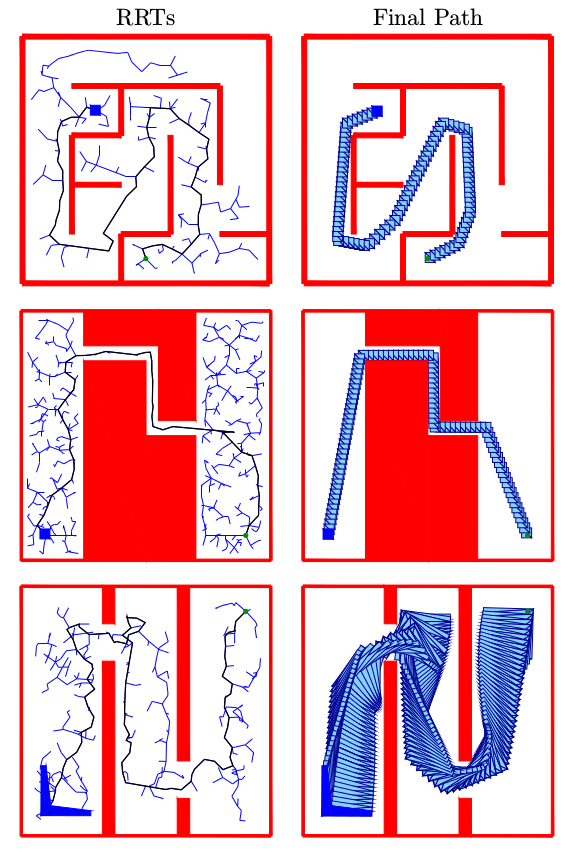
\includegraphics[width=0.4\textwidth]{figures/rrt_connect}
	\caption{RRT-Connect Example}
	\label{fig:rrt_connect}
\end{figure}
% section path_planning (end)

\section{Path optimization} % (fold)
\label{sec:path_optimization}
Due to the speed at which the points are received, the incremental movements of the robot tend to be small, as said above. Therefore, there is little room for path optimization. However given two Q configurations, an interpolation between them is computed.\\

A natural cubic interpolation as the one showed in figure \ref{fig:cubic interpolation}, is carried out. The number of interpolated steps has to be specified so that a higher number means more smoothness but also more path time and lower speed, and vice versa.

\begin{figure}[!hb]
	\centering
	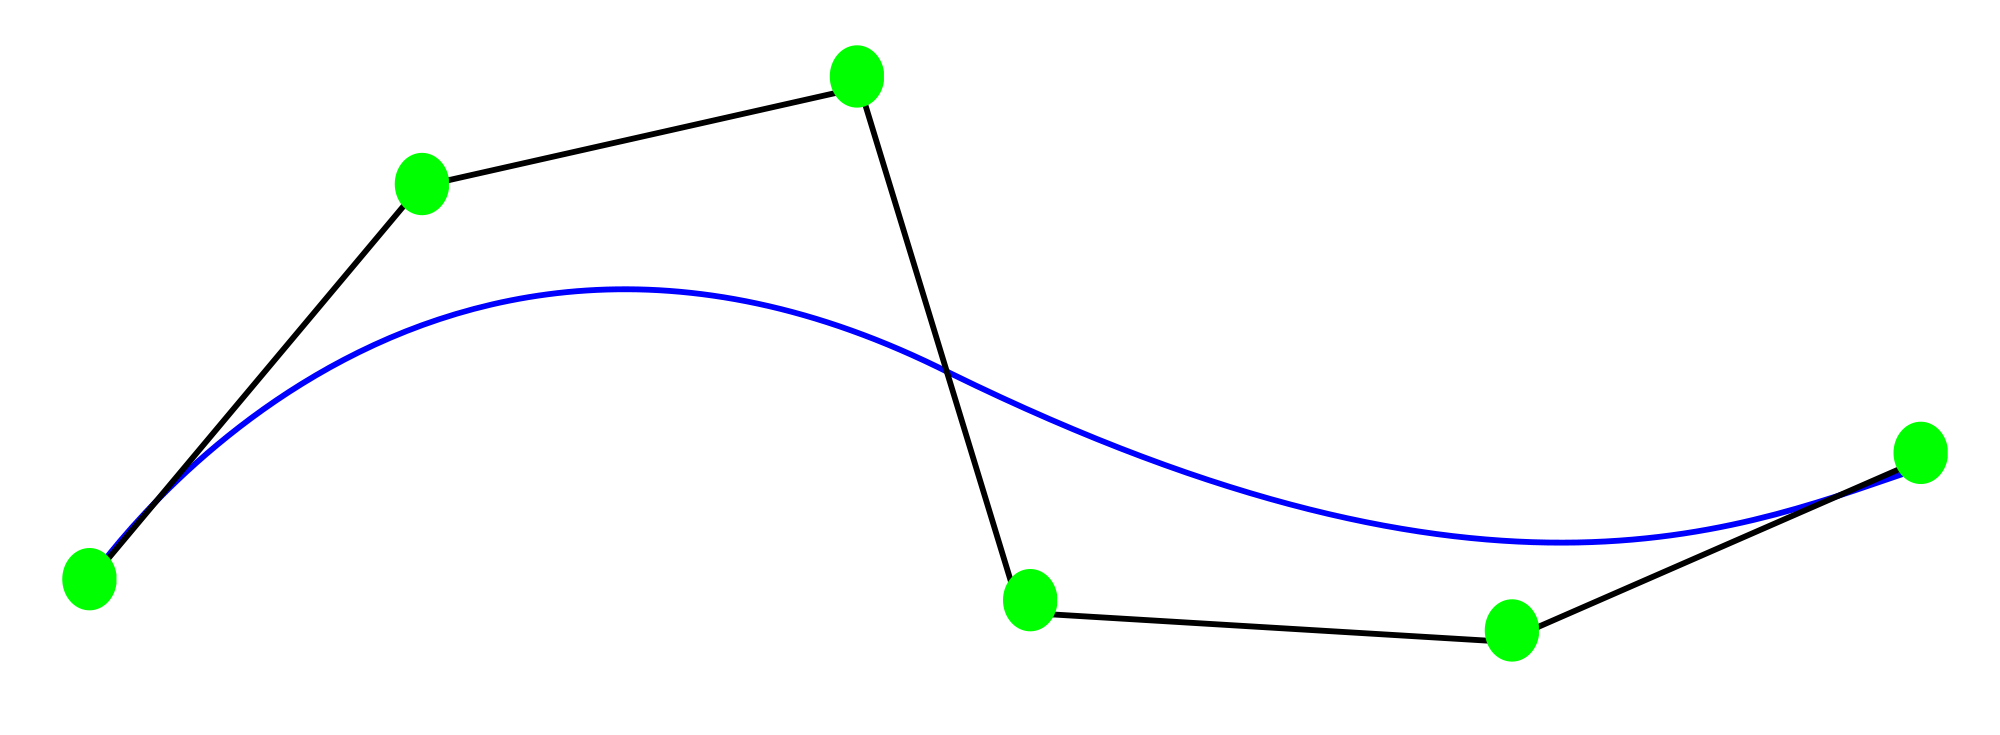
\includegraphics[width=0.8\textwidth]{figures/cubic_interpolation}
	\caption{Cubic interpolation}
	\label{fig:cubic interpolation}
\end{figure}
% section path_optimization (end)

\section{Implementation} % (fold)
\label{sec:implementation_pathplanning}
In the figure \ref{fig:path_planning_flowchart} the flow diagram of this ROS node is showed. The whole node has been developed making use of the ROS and RobWork libraries, and employing the predefined methods offered by them adjusted to best suit the goal.
\begin{figure}[!hb]
	\centering
	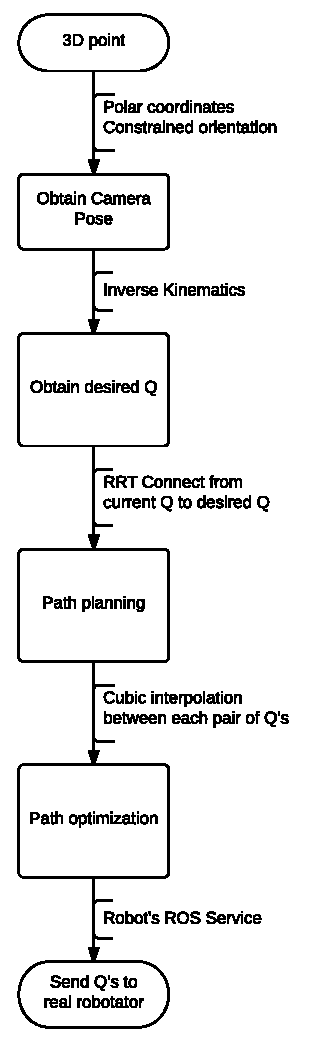
\includegraphics[height=16cm]{figures/path_planning_flowchart}
	\caption{Flowchart of the path planning method}
	\label{fig:path_planning_flowchart}
\end{figure}

	\subsection{Constrained planning} % (fold)
	\label{sub:contrained_planning_implementation}
	\subsubsection{X, Y and Z coordinates} % (fold)
	\label{subsub:x_y_and_z_coordinates}
	To reduce the degrees of freedom of the problem two constraints are applied:
	\begin{enumerate}
		\item The world reference frame is located in the base of the robot.
		\item The camera will keep a fixed distance in the Z axis from the object.
	\end{enumerate}
	The reason for the first assumption is explained later, while the argument for the second is to constrain the problem to a smaller set of solutions. 
	Now, all the possible camera poses lie on the surface of a sphere whose center is the target and whose radius is the specified distance between the camera and the object in Z.
	In order to minimize and control the robot displacement, the most suitable pose has been determined to be that in which the center of the camera belong to the plane formed by the robot's Z base axis and the tracked point. 
	This reduces the set of solutions to the circumference resulting of intersecting the defined plane and the sphere.
	The fact that the robot is now constrained to this plane, makes inverse kinematics solver more likely to find a possible configuration.\\

	So based on the assumption of fixed distance in Z between the target and the camera, a better way to express its pose would be one which includes this distance as a variable.  
	This means that a distance that allows to keep the tracked object far enough to have its whole shape in the image, but close enough for a valid triangulation, must be defined.
	For this reason, and this is only valid when the robot's base is centered in the world reference frame, cylindrical coordinates are used to express the pose vector from \ref{eq:pose_cartesian_coordinates} as in \ref{eq:pose_polar_coorinates};
		\begin{equation}
		\label{eq:pose_polar_coorinates}
			Pose = [r,\alpha,z,R,P,Y]
		\end{equation}
	So transforming the 3D point of the tracked object to cylindrical coordinates it can be obtained the desired pose angle $\alpha$ and the radius $r$ from the robot's base axis. 
	The angle $\alpha$ is the same based on the first assumption and because we want the camera to be in the plane formed by the robot's z base axis and the tracked point. 
	The radius can be calculated as the actual $r_object$ minus the desired distance to the object. Is minus because we want it in the direction of the robot's base. 
	So the camera's pose is now defined as:
		\begin{equation}
		\label{eq:cameras_pose_noRPY_noZ}
			Pose_{camera} = [r_{object},\alpha_{object},z,R,P,Y]
		\end{equation}
	The height keeps being an unknown but, and due to the fact that the next position of the object is unknown, no predictions about the height can be made. 
	For this reason the camera's height is assumed to be the same as the tracked object. This assumption included in the equation \ref{eq:cameras_pose_noRPY_noZ} gives:
		\begin{equation}
			\label{eq:cameras_pose_noRPY}
			Pose_{camera} = [r_{object},\alpha_{object},z_{object},R,P,Y]
		\end{equation}
	% subsection x_y_and_z_coordinates (end)
	\subsubsection{R, P and Y angles} % (fold)
	\label{subsub:r_p_and_y_angles}
	Knowing that the plane ZY of the reference frame of the camera will be contained in the theoretical plane expressed previously, its Z axis must point to the target.

	******************** 

	Assuming that the X and Y axis are parallel to the robot's base frame the angles can be obtained easily.
	This assumption is consistent with the same idea applied in the obtainment of the height. 
	The future state of the object is unknown and due to the robustness of the system is searched, the camera would look directly to the object.\\

	This implies that the camera's Z axis must look to the point, so the roll (R) should be the transformation from the robot's base to the camera plus the angle from the polar coordinates calculated previously.
	Regarding the the pitch (P) and the yaw (Y), is more likely to find a valid state solution if these are parallel to the robot's base reference frame. 
	The camera can be put in another alignment than the base which would include an offset in R,P and/or Y, but supposing the axis are aligned, the final camera's pose is:

	******************************

		\begin{equation}
			\label{eq:cameras_pose}
			Pose_{camera} = [r_{object},\alpha_{object},z_{object},\alpha_{object},0,0]
		\end{equation}
	% subsubsection r_p_and_y_angles (end)
	% subsection contrained_planning (end)

	\subsection{RRT-Connect} % (fold)
	\label{sub:rrt_connect_implementation}
	\subsubsection{Metric} % (fold)
	\label{sub:metric}
	The metric is the way two different robot's configurations are measured. This will define the behavior of the planner along with the extension [\ref{sub:extension}]. For this project, the $Euclidean distance$ has been chosen, due to the balance in the measure that all the joints produce. This is defined by:
	\begin{equation}
		d=\sqrt{\sum_i^N q_i^2}
	\end{equation}
	% subsection metric (end)

	\subsubsection{Extension} % (fold)
	\label{sub:extension}
	The extension is the distance from which another configuration in consider as a neighbor. This distance depends on how the metrics has been defined.
	% subsection extension (end)

	\subsubsection{Collision detector} % (fold)
	\label{sub:collision_detector}
	The collision detector is the strategy used to define when two objects are colliding. Based on our criteria of fast detection and that only simple geometries are found in our work cell, the Yaobi strategy \cite{Yaobi} has ben chosen. Yaobi, as defined in the webpage,  "is a small collision detection library for arbitrary meshes. I was inspired by the excellent libraries PQP and Opcode, and hopefully I have managed to combine the best parts of both: oriented bounding boxes (OBBs) and hybrid tree structure. Like PQP, Yaobi uses an OBB-tree to model objects. PQP takes this representation to its limit, surrounding each triangle with a single leaf-OBB. Yaobi instead uses the hybrid approach of Opcode, where leaf-nodes surround two triangles each (TriNodes). The hybrid approach not only saves a lot of memory, it also makes collision queries run faster. Benchmarks show that Yaobi is between 2.5 to 3 times faster than PQP. For near convex objects, Opcode is slightly faster, but for curved objects and small objects inside larger ones, Yaobi gets the upper hand."
	% subsection collision_detector (end)
	\subsubsection{Sampler} % (fold)
	\label{sub:sampler}
	The sampler defines how the new configurations need to be created in the $C_{free}$. In this case the sampler chosen has been $Uniform$. This is due to the not patterned geometries so, for example, there is no preference in the direction the new configuration are going to be created.
	% subsection sampler (end)
% subsection rrt_connect (end)
\subsection{Path optimization} % (fold)
\label{sub:path_optimization_implementation}
Path optimization some interpolations have been tested. 
From the Circular Interpolator until the Linear Interpolator, the one with best and smother results has been the Cubic Spline Interpolator in its variance natural spline.
Due to the robot's speed was fixed and limited, the factor to define the differential step has been the number of divisions made between two robot's configuration. 
During this project a number of 4 intermediate Q's has been used.
% subsection path_optimization (end)


% section implementation (end)

\section{Experimental results} % (fold)
\label{sec:experimental_results_pathplanning}

% section experimental_results (end)

\section{Conclusions} % (fold)
\label{sec:conclusions_pathplanning}
A simple query path planning RRT-Connect, with constrained planning and path optimization has been implemented. \\

On one hand, the assumptions taken when calculating the constrained robot's configuration has been proven to be valid for our experiments. 
Furthermore, the RRT-Connect not only has shown to be valid for the project but also has extend our knowledge in this topic which is inside of the course's scope.
On the path optimization part, the natural cubic splines have proved to be a good and useful tool when interpolating two Q's, smoothing the robot's movements. \\

On the other hand, not only everything has been implemented inside a ROS node and using the RobWork libraries so a further understanding of those has been achieved, but also two auxiliar plugin, the $server point$ and the $Robwork plugin$, has been implemented in parallel so this node could have been tested without depending on the others.

TODO: This is too positive, add some of the experiments conclusions
% section conclusions (end)

% chapter path_planning (end)
	\chapter{Calibration} % (fold)
\label{cha:calibration}

\section{Camera calibration} % (fold)
\label{sec:camera_calibration}

% section camera_calibration (end)

\section{Robot calibration} % (fold)
\label{sec:robot_calibration}

% section robot_calibration (end)

% chapter calibration (end)
	\chapter{Experiments} % (fold)
\label{cha:experiments}

% chapter experiments (end)

	%!TEX root = ../report.tex
\chapter{Discussion}
\label{chap:discussion}
On an overall level, the system is working as intended. 
However, through the pipeline formed by the nodes structure there are several potential sources of errors which have to be compensated for or at least kept in mind regarding further work.

The tasks carried out through this pipeline could be summarized as a) acquisition of the stereo images; b) object detection in each image; c) reconstruction of the original 3D point; d) estimation of the true position based on previously measured points and e) obstacles avoidance by generation of safe paths around them.
Some of the more troubling steps on the system flow are discussed below.

First the camera calibration is not entirely accurate.
Undistorted images contain some pixel error that, even though are small, will be increased through the triangulation process.

The ball detection algorithm is not perfect either.
If, for example, the ball is moved quickly, it becomes blurry in the images and longer appears as a circle.
If the ball is illuminated that can have a similar effect.
Even though the detection algorithm still finds the ball, its center of mass may be imprecise by some pixels.
The further away from the cameras the ball is, the greater the error becomes.
The 3D position of the ball is based on the camera calibration and 2D detection, so any errors in the first stage will propagate further down the pipeline.

Regarding the general speed of the system, the bottleneck is the \emph{balltracker node}. 
This node subscribes to the cameras, which are able to emit images at around 25 frames per second, however, the node only works at 3 Hz. 
This has been partially solved by two different means: (1) the node was changed to subscribe to the compressed images instead of the raw image and (2) the node processes each callback in a different thread doing this node multi threading. 
These improvements give as a result an enhanced frame rate of 5 to 10 Hz, but still far from the original 25 Hz that would make the robot perform in a more natural way.
 
The robot remains uncalibrated but as long as the error described in Section~\ref{sec:joint_error} prevails, that will certainly be the dominant one. The error is particularly pronounced if the ball is not moved very slowly, forcing large jumps in joint angles. Once the PA10 robot moves as it is supposed to, the robot error might be evaluated more thoroughly.

% For future work the first task would probably be to design a way to work around the problem with setting joint configurations which are too far from the previous. Once that is done, the robot performance can be judged more easily...

	%!TEX root = ../report.tex

\chapter{Conclusions} % (fold)
\label{cha:conclusions}
As a general conclusion, the developed system has been successfully tested in both simulation and the workcell, and subjected to experiments to measure the magnitude of the errors in the performance, as showed in Chapter \ref{cha:experiments}.
It has proved robustness and reliability, although certain limits imposed by the robot conditions have constrained the goodness of the final results. Some specific conclusions and further work are discussed at this point.

\section{Stereo vision}
On the vision part of the system, some main points can be highlighted.
The final implementation of the feature extraction algorithm for the image processing part, together with the specific design of the target have resulted in an illumination and background invariant detector, able to find reliably the target under changing environmental conditions.
Furthermore, the multithreading processing implemented to speed up the reception of the pictures acquired by the cameras, together with the use of the ROS message filters approximate sync policy to ensure their synchronization, have supposed a relevant enhancement of the system performance.
However, something that might be left as further work could be the application of the epipolar geometry theory to the correspondence problem in the detection part, in order to make it faster and more accurate as a previous step to the triangulation. 
Now two separate detection processes are carried out in each image, which work correctly, even though the epipolar constraint is not checked for the output coordinates.

\section{Trajectory prediction}
Following the vision part of the system, a Kalman filter was used in order to predict the trajectory of the object being tracked.\\

The choice of a Kalman filter instead of any others proved good and fast enough even though the movement being tracked was a random movement performed by a human instead of a free falling object or something similar. Actually, for being such a random movement, the covariances computed proved to be good enough, as the filter was able to predict the movement with an error up to 30 cm according to figure \ref{fig:ball_kalman_error}.

\section{Path planning}
A simple query path planning RRT-Connect, with constrained planning and path optimization has been implemented. \\

On one hand, the assumptions made when calculating the constrained robot's configuration generation have been proved to be valid for our experiments. 
Furthermore, the RRT-Connect not only has showed to be valid for the project but also has extended our knowledge in this topic, which is inside of the scope of this course.
On the path optimization part, the natural cubic splines have proved to be a good and useful tool when interpolating two Q's, smoothing the robot movements. Everything has been implemented inside a ROS node and using the RobWork libraries so a further understanding of those has been achieved, but also two auxiliary plugins, the $server point$ and the $Robwork plugin$, has been implemented in parallel so that this node could be tested without depending on the others.\\

On the other hand, speed problems have been found making the robot move slow. Also the main problem is in the inverse kinematics solver where a solution is not always found. Despite that the node has shown to be useful and effective.


% chapter conclusions (end)
	%!TEX root = ../report.tex
\begin{thebibliography}{9}

\bibitem{suzuki}
	Satoshi Suzuki, Keiichia Be,
	\emph{Topological structural analysis of digitized binary images by border following},
	Computer Vision, Graphics, and Image Processing 30, 32-46,
	1985.
	
\bibitem{kalman}
	R. E. Kalman,
	\emph{A New Approach to Linear Filtering and Prediction Problems},
	Journal of Basic Engineering 82, (Series D): 35-45,
	1960.

\bibitem{RRTConnect}
	James J. Kuffner, Jr., Steven M. LaValle,
	\emph{RRT-Connect: An Efficient Approach to Single-Query Path Planning},
	Proc. 2000 IEEE Int’l Conf. on Robotics and Automation,ICRA, 2000.

\bibitem{Zhang}
	Zhengyou Zhang,
	\emph{Flexible Camera Calibration By Viewing a Plane From Unknown Orientations},
	Microsoft Research, One Microsoft Way, Redmond, WA 98052-6399, USA
	1998.

\bibitem{Hartley}
	Richard Hartley, Andrew Zisserman
	\emph{Multiple View Geometry in Computer Vision},
	$2^{\circ}$ Edition, Cambridge.

\bibitem{Brown}
	Duane C. Brown
	\emph{Decentering Distortion of Lenses},
	D. Brown Associates, Inc.

\end{thebibliography}

\end{document}
